% Copyright 2004 by Till Tantau <tantau@users.sourceforge.net>.
%
% In principle, this file can be redistributed and/or modified under
% the terms of the GNU Public License, version 2.
%
% However, this file is supposed to be a template to be modified
% for your own needs. For this reason, if you use this file as a
% template and not specifically distribute it as part of a another
% package/program, I grant the extra permission to freely copy and
% modify this file as you see fit and even to delete this copyright
% notice. 

\documentclass{beamer}

% There are many different themes available for Beamer. A comprehensive
% list with examples is given here:
% http://deic.uab.es/~iblanes/beamer_gallery/index_by_theme.html
% You can uncomment the themes below if you would like to use a different
% one:
%\usetheme{AnnArbor}
%\usetheme{Antibes}
%\usetheme{Bergen}
%\usetheme{Berkeley}
%\usetheme{Berlin}
%\usetheme{Boadilla}
%\usetheme{boxes}
\usetheme{CambridgeUS}
%\usetheme{Copenhagen}
%\usetheme{Darmstadt}
%\usetheme{default}
%\usetheme{Frankfurt}
%\usetheme{Goettingen}
%\usetheme{Hannover}
%\usetheme{Ilmenau}
%\usetheme{JuanLesPins}
%\usetheme{Luebeck}
%\usetheme{Madrid}
%\usetheme{Malmoe}
%\usetheme{Marburg}
%\usetheme{Montpellier}
%\usetheme{PaloAlto}
%\usetheme{Pittsburgh}
%\usetheme{Rochester}
%\usetheme{Singapore}
%\usetheme{Szeged}
%\usetheme{Warsaw}

\usepackage[USenglish]{babel}
\usepackage[latin1]{inputenc}
\usepackage{booktabs}
\usepackage[scale=2]{ccicons}
\usepackage{pgfplots}
\usepackage{xspace}
\usepackage{enumerate}
\usepackage{amsthm}
\usepackage[alf]{abntex2cite}
%\usepackage{subcaption}
%\usepgfplotslibrary{dateplot}
\usepackage{graphicx}
\usepackage{mathtools}
%\DeclarePairedDelimiter\abs{\lvert}{\rvert}%
%\usepackage{latexsym}
%\usepackage{amsmath}
%\usepackage[T1]{fontenc}
%\usepackage{fetamont}
%\usepackage{mathrsfs}
\usepackage{subfigure}
%\usepackage{chngcntr}
%\usepackage{fancyhdr}
%\usepackage{xmpmulti}
%\usepackage{animate}
\usepackage{ragged2e}
\usepackage{pdfpages}
\usepackage{epstopdf}

\setbeamertemplate{caption}[numbered]
%\setbeamertemplate{footline}[]{}
\setbeamertemplate{navigation symbols}{}
\setbeamertemplate{caption}{\raggedright\insertcaption\par}



%\setbeamertemplate{footline}
%{
%	\leavevmode%
%	\hbox{%
%		\begin{beamercolorbox}[wd=.3\paperwidth,ht=2.25ex,dp=1ex,center]{author in head/foot}%
%			\usebeamerfont{author in head/foot}\insertshortauthor
%		\end{beamercolorbox}%
%		\begin{beamercolorbox}[wd=.4\paperwidth,ht=2.25ex,dp=1ex,center]{title in center/foot}%
%			\usebeamerfont{title in head/foot}\insertshorttitle\hspace*{3em}
%		\end{beamercolorbox}%
%		\begin{beamercolorbox}[wd=.3\paperwidth,ht=2.25ex,dp=1ex,center]{conf and page/foot}%
%			\usebeamerfont{conf and page/foot}\insertshortdate\hspace*{3em}
%			\insertframenumber{} / \inserttotalframenumber\hspace*{1ex}
%		\end{beamercolorbox}}%
%	\vskip0pt%
%}



\title[Cryptocurrencies Transactions Advisor]{Cryptocurrencies Transactions Advisor Using a Genetic Mamdani-type Fuzzy Rules Based System}

% A subtitle is optional and this may be deleted
%\subtitle{Optional Subtitle}

\author{T.~Tupinambas\inst{1} \and R.~Le�o\inst{2} \and A.~Lemos\inst{1}}
% - Give the names in the same order as the appear in the paper.
% - Use the \inst{?} command only if the authors have different
%   affiliation.

\institute[] % (optional, but mostly needed)
{
	\inst{1}%
	Graduate Program in Electrical Engineering\\
	Federal University of Minas Gerais
	\and
	\inst{2}%
	Cadence Design Systems, Inc.}
% - Use the \inst command only if there are several affiliations.
% - Keep it simple, no one is interested in your street address.

\date[FUZZ-IEEE, 2018]{IEEE International Conference on Fuzzy Systems, 2018}
% - Either use conference name or its abbreviation.
% - Not really informative to the audience, more for people (including
%   yourself) who are reading the slides online

\subject{Theoretical Computer Science}
% This is only inserted into the PDF information catalog. Can be left
% out. 

% If you have a file called "university-logo-filename.xxx", where xxx
% is a graphic format that can be processed by latex or pdflatex,
% resp., then you can add a logo as follows:

% \pgfdeclareimage[height=0.5cm]{university-logo}{university-logo-filename}
% \logo{\pgfuseimage{university-logo}}

% Delete this, if you do not want the table of contents to pop up at
% the beginning of each subsection:
\AtBeginSubsection[]
{
	\begin{frame}<beamer>{Outline}
	\tableofcontents[currentsection,currentsubsection]
\end{frame}
}

% Let's get started
\begin{document}

{
	\setbeamertemplate{footline}{} 
	\begin{frame}
	\titlepage
\end{frame}
}
\addtocounter{framenumber}{-1}
%
%\begin{frame}
%  \titlepage
%\end{frame}

\begin{frame}{Outline}
\tableofcontents
% You might wish to add the option [pausesections]
\end{frame}

% Section and subsections will appear in the presentation overview
% and table of contents.

%------------------------------------------------SECTION---------------------------------
\section{Motivation} 
%------------------------------------------------SUBSECTION------------------------------

\subsection{Sensor Market}

\begin{frame}
\frametitle{Growth}
Global Sensor Market is expected to garner USD 241 billion by 2022, registering a CAGR of 11.3 \% during the forecast period 2016 - 2022. Sensor is a device that detects physical input such as light, heat, motion, moisture, pressure, or any other entity, and responds by producing an output on a display or transmits the information in electronic form for further processing. The sensors find their applications in various industries such as electronics, IT \& telecommunication, automotive and healthcare among others. 

In the current scenario, smart grid, smart homes, smart water networks, intelligent transportation are infrastructure systems that connect our world are trending. These systems are assembled through the use of sensors, and the entire physical infrastructure is closely coupled with information and communication technologies. Intelligent monitoring and management can be achieved via the usage of networked embedded systems, in which devices are interconnected to transmit useful measurement information and control instructions via distributed sensor networks. 


\end{frame}
\frametitle{Growth}

%------------------------------------------------

\begin{frame}
\frametitle{Sensor Market}

The global industrial sensors market to grow at a CAGR of 7.87\% during the period 2018-2022.

Global Industrial Sensors Market 2018-2022, has been prepared based on an in-depth market analysis with inputs from industry experts. The report also includes a discussion of the key vendors operating in this market. To calculate the market size, the report considers the revenue generated from the use of different types of sensors across different industries.


The latest trend gaining momentum in the market is the increasing demand for remote monitoring. The advent of the industrial IoT is expected to represent the biggest opportunity for the development of industrial sensors across different end-user industries.

\end{frame}

%------------------------------------------------

\begin{frame}
\frametitle{Market Size}

\begin{figure}
\centering
%\caption{}t
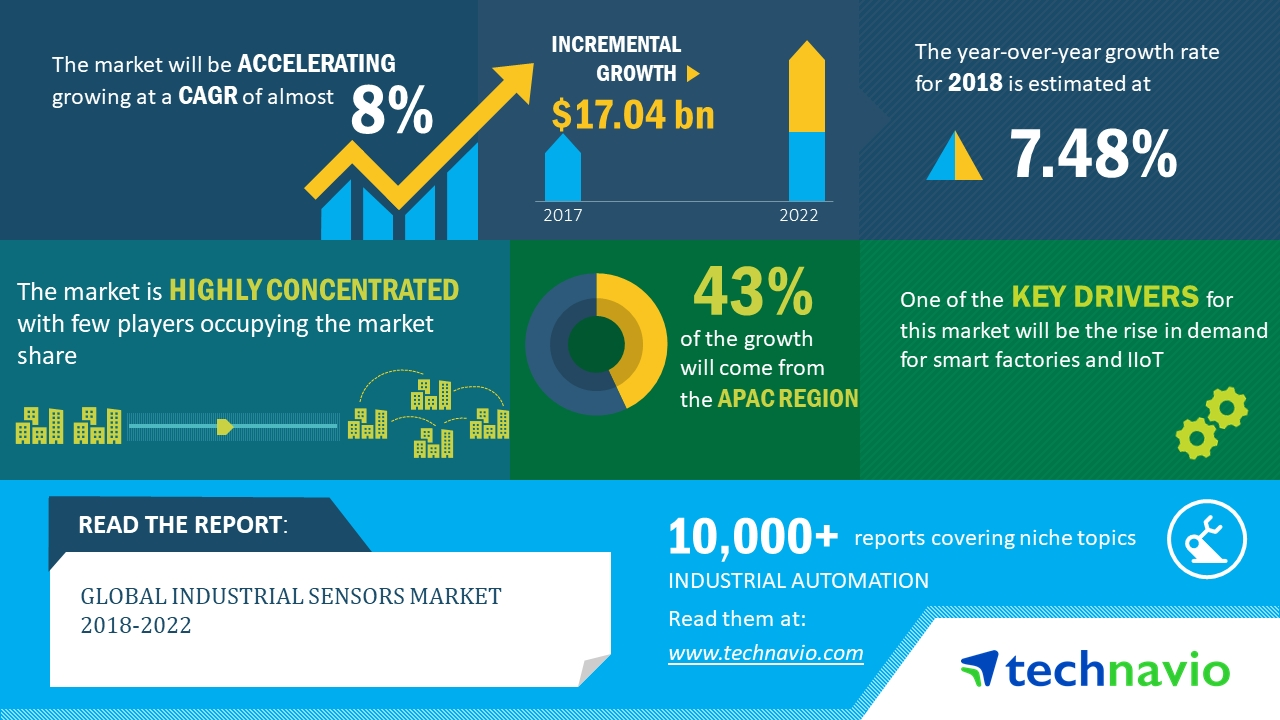
\includegraphics[width=0.9\textwidth]{images/global_ind_sensor.jpg}
\par
\vspace{0.3cm}
\tiny Source: \href{https://coinmarketcap.com/all/views/all/}{https://coinmarketcap.com/all/views/all/} Accessed on: Jul 01, 2018 9:00 PM UTC
\end{figure}

\end{frame}
%------------------------------------------------

\begin{frame}
\frametitle{Sensor network complexity}

More sensors, more complex networks.

Unsynchronized measurements

Time delays

Aperiodic sampling

\end{frame}
%------------------------------------------------

\begin{frame}
\frametitle{Examples}

Big data, HAR with the use of accelerometers and girometers.


\end{frame}
%------------------------------------------------

\begin{frame}
\frametitle{Examples}

State estimation

\end{frame}


%------------------------------------------------
%
%%\section{Refer�ncias}
%\begin{frame}
%\frametitle{References}
%\bibliography{biblio}
%\end{frame}

\end{document}


